\documentclass[12pt,letterpaper]{book}
\usepackage[spanish]{babel}
\usepackage{graphicx}
\usepackage[top=2cm,bottom=2cm,left=3cm,right=2cm]{geometry}
\usepackage{fancyhdr}   % Paquete para encabezados o pies de página.

\usepackage{emptypage}  % Paquete para la prevensión de aparición 
                        % de pies de página, encabezados y numeración.

\usepackage{float}      % Paquete para la adecuación de cuadros y tablas.

\usepackage{longtable}  % Paquete que permite la construcción de tablas
                        % que abarque mas de una página.

\usepackage{apacite}    % Paquete que ofrece el soporte de la citación 
                        % estilo APA.
                    
\usepackage{blindtext}
\usepackage{enumitem}   % opcional

\usepackage{docstyle}

\begin{document}
    \newgeometry{top=2cm,bottom=2cm,left=2cm,right=2cm}
\begin{titlepage}
    \begin{minipage}{2.7cm}
        \begin{center}
            
\includegraphics[width=3cm,height=3cm]{img/logo_universidad.png}
        \end{center}
    \end{minipage}
    \hfill
    \begin{minipage}{11cm}
        \begin{center}
            \large{ \textbf{\MakeUppercase{\nombreUniversidad}} }\\
            \normalsize{ \textbf{\MakeUppercase{\nombreFacultad}} }\\
            \small{ \textbf{\MakeUppercase{\nombreCarrera}} }
        \end{center}
    \end{minipage}
    \hfill
    \begin{minipage}{3.0cm}
        \begin{center}
            
\includegraphics[width=3.0cm,height=3.0cm]{img/logo_facultad.png}
        \end{center}
    \end{minipage}
    \vspace{5cm}\\
    \begin{center}
        \MakeUppercase{\nombreProyecto}
    \end{center}
    \vspace{4cm}
    \descripcion\\

    \vspace{2cm}
    \textnormal{\textbf{Presentado por:} \nombreAutor}\\

    \vspace{0.3cm}
    \textnormal{\textbf{Tutor:} \nombreTutor}\\

    \vspace{3.5cm}
    \begin{center}
        \textbf{\MakeUppercase{\nombreCiudadPais}}\\
        \fecha
    \end{center}
\end{titlepage}
\restoregeometry
    \frontmatter
             
\chapter{Dedicatoria}
Duis fringilla tristique neque. Sed interdum libero ut metus.
Pellentesque placerat. Nam rutrum augue a leo. Morbi sed 
elit sit amet ante lobortis sollicitudin.Praesent blandit 
blandit mauris. Praesent lectus tellus, aliquet aliquam,
luctus a, egestas a, turpis.Mauris lacinia lorem sit amet
ipsum. Nunc quis urna dictum turpis accumsan semper.iii
    \chapter{Agradecimientos}
Lorem ipsum dolor sit amet, consectetuer adipiscing elit. 
Etiam lobortis facilisis sem. Nullam necmi  et  neque  
pharetra  sollicitudin.  Praesent  imperdiet  mi  nec  
ante.  Donec  ullamcorper,  felis  nonsodales commodo, 
lectus velit ultrices augue, a dignissim nibh lectus 
placerat pede. Vivamus nuncnunc, molestie ut, ultricies 
vel, semper in, velit. Ut porttitor. Praesent in sapien.
Lorem ipsum dolorsit amet, consectetuer adipiscing elit. 
Duis fringilla tristique neque. Sed interdum libero ut metus.
Pellentesque placerat. Nam rutrum augue a leo. Morbi sed 
elit sit amet ante lobortis sollicitudin.Praesent blandit 
blandit mauris. Praesent lectus tellus, aliquet aliquam,
luctus a, egestas a, turpis.Mauris lacinia lorem sit amet
ipsum. Nunc quis urna dictum turpis accumsan semper.iii

Praesent in sapien. Lorem ipsum dolorsit amet, consectetuer 
Duis fringilla tristique neque. Sed interdum libero ut metus.
Pellentesque placerat. Nam rutrum augue a leo. Morbi sed 
elit sit amet ante lobortis sollicitudin.Praesent blandit 
blandit mauris. Praesent lectus tellus, aliquet aliquam,
luctus a, egestas a, turpis.Mauris lacinia lorem sit amet
ipsum. Nunc quis urna dictum turpis accumsan semper.iii
    \mainmatter     
    \tableofcontents
    \listoffigures
    \listoftables
    \chapter{Introducción}

\begin{center}
    \textit{En que consiste este capítulo}
\end{center}

\blindtext\\ % Relleno de texto

\blindtext\\ % Relleno de texto

Fringilla tristique neque. Sed interdum libero ut metus.
Pellentesque placerat. Nam rutrum augue a leo. Morbi sed 
elit sit amet ante.\\

Duis fringilla tristique neque. Sed interdum libero ut metus.
Pellentesque placerat. Nam rutrum augue a leo. Morbi sed 
elit sit amet ante lobortis sollicitudin.Praesent blandit 
blandit mauris. Praesent lectus tellus, aliquet aliquam,
luctus a, egestas a, turpis.Mauris lacinia lorem sit amet
ipsum. Nunc quis urna dictum turpis accumsan semper. Figura
\ref{fig:ejemplo}.\\

\begin{figure}[H]
    \centering
        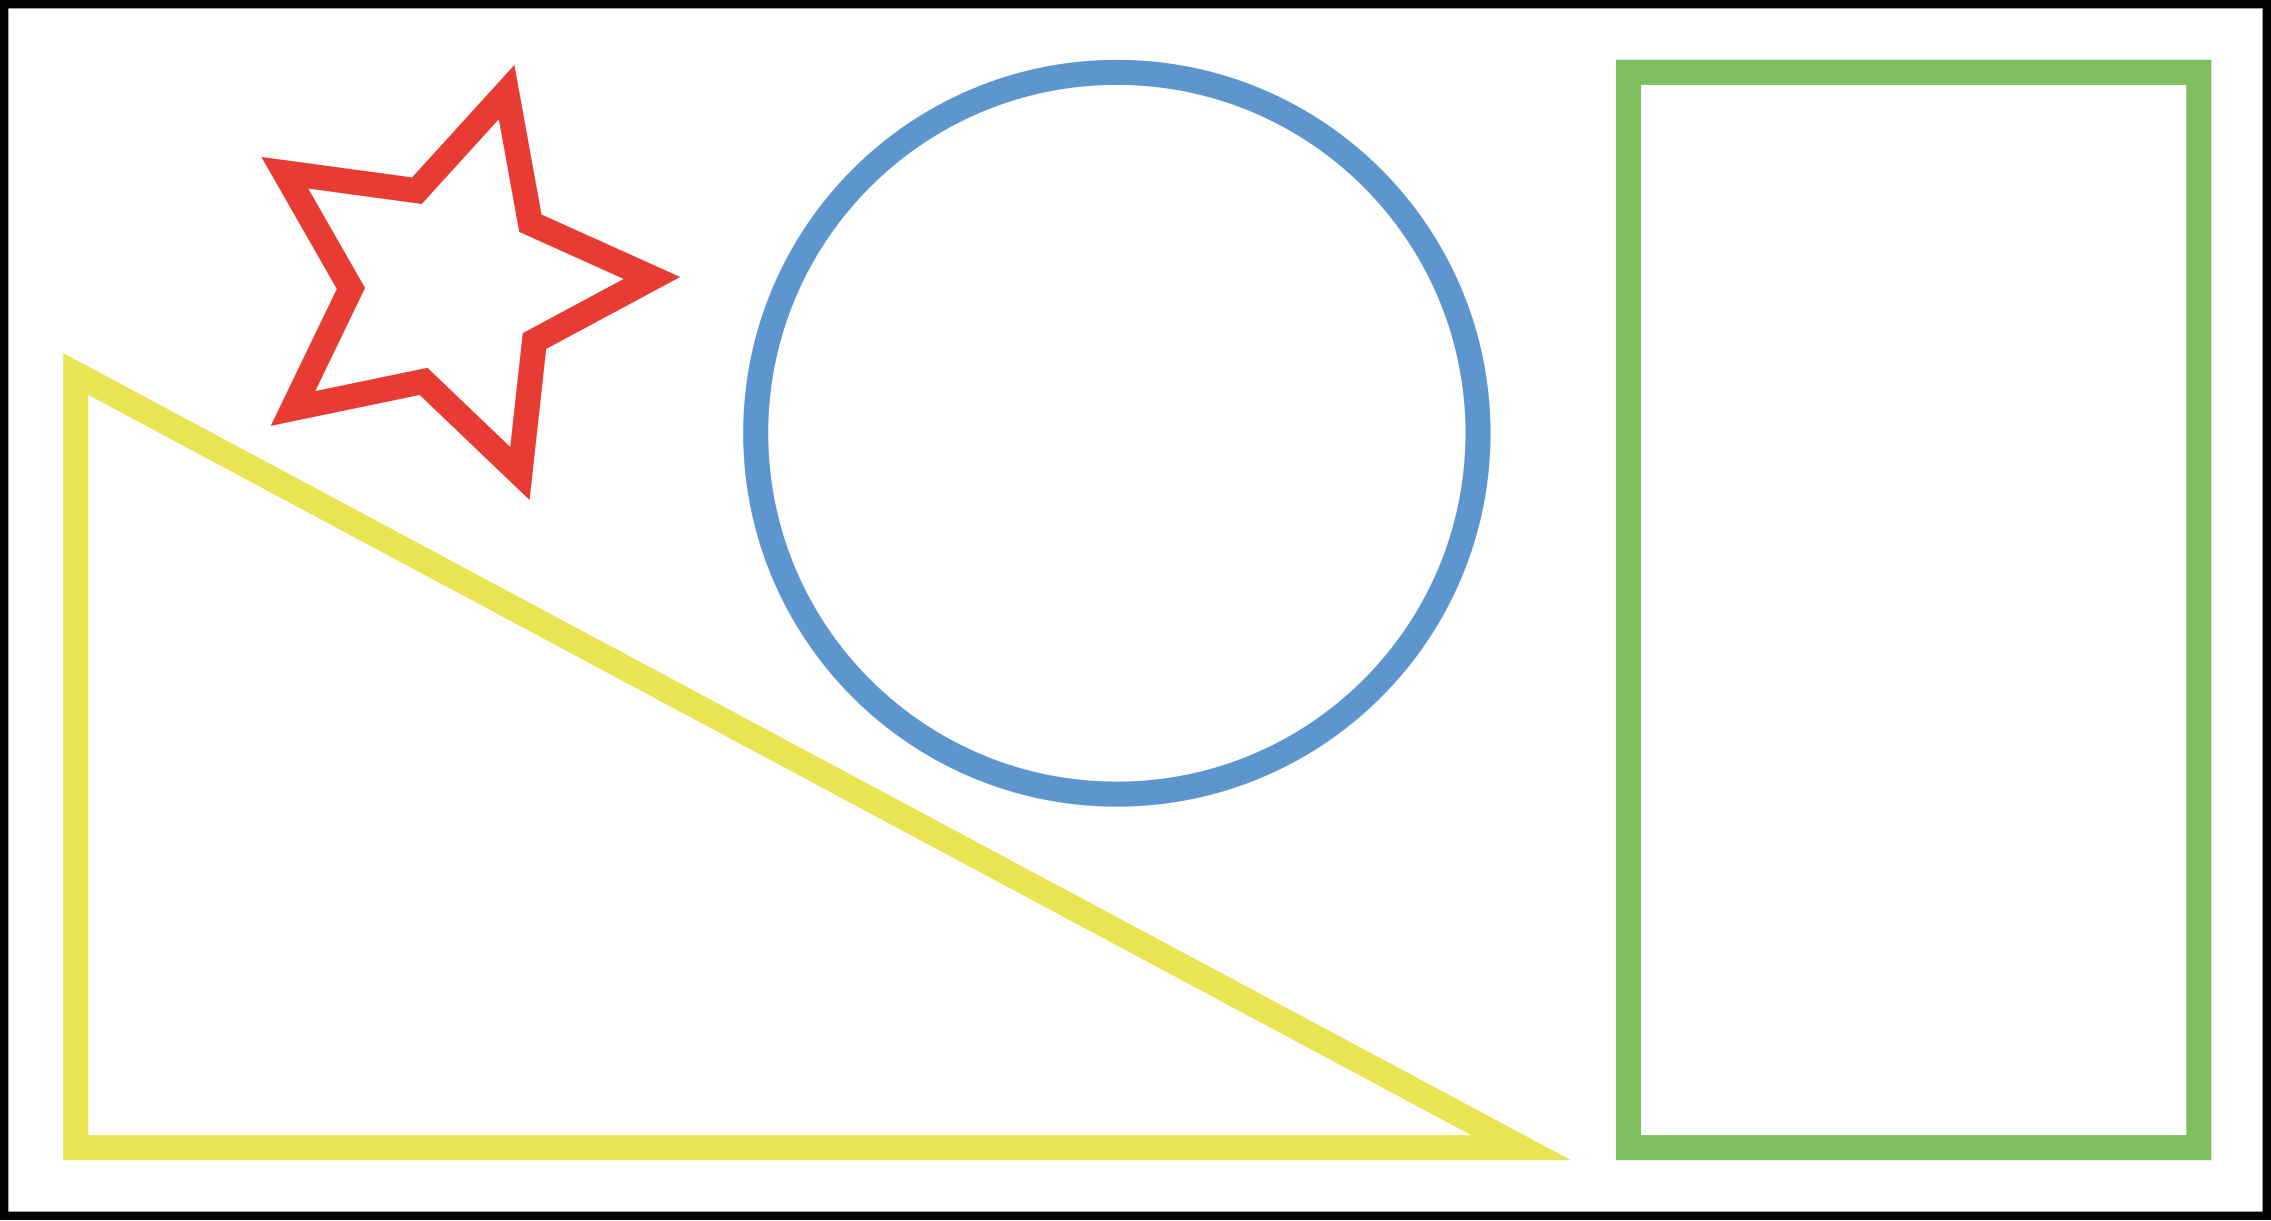
\includegraphics[width=8cm]{img/figura_ejemplo.png}
    \caption{Explicación de la figura (Aquí)}
    Fuente: \textit{Libro Ejemplo} por \citeA[p.~5]{book:ejemplo_simple}
    \label{fig:ejemplo}
\end{figure}

Stique neque. Sed interdum libero ut metus.
Pellentesque placerat. Nam rutrum augue a leo. Morbi sed 
elit sit amet ante lobortis sollicitudin.Praesent blandit 
blandit mauris. Praesent lectus tellus, aliquet aliquam,
luctus a, egestas a, turpis.Mauris lacinia lorem sit amet
ipsum. Nunc quis urna dictum turpis accumsan semper. Cuadro
\ref{cuadro:ejemplo}.\\

\begin{table}[H]
    \centering
    \caption{Título del cuadro}
    \vspace{0.5cm}
    \label{cuadro:ejemplo}
    \begin{tabular}{c|c|c|c|}
        \cline{2-4}
                                              & \textbf{Columna 1} & \textbf{Columna 2} & \textbf{Columna 3} \\ \hline
        \multicolumn{1}{|c|}{\textbf{Fila 1}} & item               & item               & item               \\ \hline
        \multicolumn{1}{|c|}{\textbf{Fila 2}} & item               & item               & item               \\ \hline
        \multicolumn{1}{|c|}{\textbf{Fila 3}} & item               & item               & item               \\ \hline
    \end{tabular}
    \begin{center}
        Nota. Cuadro extraído de \textit{Libro Ejemplo} por \citeA[p.~20]{book:ejemplo_simple}
    \end{center}
\end{table}

\blindtext\\ % Relleno de texto

Stique neque. Sed interdum libero ut metus.
Pellentesque placerat. Nam rutrum augue a leo. Morbi sed 
elit sit amet ante lobortis sollicitudin.Praesent blandit 
blandit mauris. Praesent lectus tellus, aliquet aliquam,
luctus a, egestas a, turpis.Mauris lacinia lorem sit amet
ipsum. Nunc quis urna dictum turpis accumsan semper. Cuadro
\ref{cuadro:cuadro_largo_ejemplo}.\\

\begin{longtable}{p{2cm}|p{3cm}|p{3cm}|p{3cm}|p{3cm}|}
    \caption{Titulo de cuadro multipágina} \label{cuadro:cuadro_largo_ejemplo} \\
    \cline{2-5}
    \multicolumn{1}{l|}{} & \multicolumn{1}{c|}{\textbf{Columna 1}} & \multicolumn{1}{c|}{\textbf{Columna 2}} & \multicolumn{1}{c|}{\textbf{Columna 3}} & \multicolumn{1}{c|}{\textbf{Columna 4}}\\ \hline
    \endfirsthead

    \multicolumn{5}{c}{{\tablename{} \thetable{} -- Continuación de cuadro previo}} \\
    \multicolumn{5}{l}{} \\
    \cline{2-5}
    \multicolumn{1}{l|}{} & \multicolumn{1}{c|}{\textbf{Columna 1}} & \multicolumn{1}{c|}{\textbf{Columna 2}} & \multicolumn{1}{c|}{\textbf{Columna 3}} & \multicolumn{1}{c|}{\textbf{Columna 4}}\\ \hline
    \endhead

    \multicolumn{5}{c}{{Continua en la siguiente página.}} \\
    \endfoot

    \multicolumn{5}{l}{} \\
    \multicolumn{5}{l}{{Nota. Cuadro extraído de \textit{Libro Ejemplo} por \citeA[p.~20]{book:ejemplo_simple} }} \\
    \endlastfoot

    \multicolumn{1}{|c|}{\textbf{Fila 1}} & Lorem ipsum dolor sit amet, consectetuer adipiscing elit. & Lorem ipsum dolor sit amet, consectetuer adipiscing elit. & Lorem ipsum dolor sit amet, consectetuer adipiscing elit. & Lorem ipsum dolor sit amet, consectetuer adipiscing elit. \\ \hline
    \multicolumn{1}{|c|}{\textbf{Fila 2}} & Lorem ipsum dolor sit amet, consectetuer adipiscing elit. & Lorem ipsum dolor sit amet, consectetuer adipiscing elit. & Lorem ipsum dolor sit amet, consectetuer adipiscing elit. & Lorem ipsum dolor sit amet, consectetuer adipiscing elit. \\ \hline
    \multicolumn{1}{|c|}{\textbf{Fila 3}} & Lorem ipsum dolor sit amet, consectetuer adipiscing elit. & Lorem ipsum dolor sit amet, consectetuer adipiscing elit. & Lorem ipsum dolor sit amet, consectetuer adipiscing elit. & Lorem ipsum dolor sit amet, consectetuer adipiscing elit. \\ \hline
    \multicolumn{1}{|c|}{\textbf{Fila 4}} & Lorem ipsum dolor sit amet, consectetuer adipiscing elit. & Lorem ipsum dolor sit amet, consectetuer adipiscing elit. & Lorem ipsum dolor sit amet, consectetuer adipiscing elit. & Lorem ipsum dolor sit amet, consectetuer adipiscing elit. \\ \hline
    \multicolumn{1}{|c|}{\textbf{Fila 5}} & Lorem ipsum dolor sit amet, consectetuer adipiscing elit. & Lorem ipsum dolor sit amet, consectetuer adipiscing elit. & Lorem ipsum dolor sit amet, consectetuer adipiscing elit. & Lorem ipsum dolor sit amet, consectetuer adipiscing elit. \\ \hline
    \multicolumn{1}{|c|}{\textbf{Fila 6}} & Lorem ipsum dolor sit amet, consectetuer adipiscing elit. & Lorem ipsum dolor sit amet, consectetuer adipiscing elit. & Lorem ipsum dolor sit amet, consectetuer adipiscing elit. & Lorem ipsum dolor sit amet, consectetuer adipiscing elit. \\ \hline  
    \multicolumn{1}{|c|}{\textbf{Fila 7}} & Lorem ipsum dolor sit amet, consectetuer adipiscing elit. & Lorem ipsum dolor sit amet, consectetuer adipiscing elit. & Lorem ipsum dolor sit amet, consectetuer adipiscing elit. & Lorem ipsum dolor sit amet, consectetuer adipiscing elit. \\ \hline    
    \multicolumn{1}{|c|}{\textbf{Fila 8}} & Lorem ipsum dolor sit amet, consectetuer adipiscing elit. & Lorem ipsum dolor sit amet, consectetuer adipiscing elit. & Lorem ipsum dolor sit amet, consectetuer adipiscing elit. & Lorem ipsum dolor sit amet, consectetuer adipiscing elit. \\ \hline    
    \multicolumn{1}{|c|}{\textbf{Fila 9}} & Lorem ipsum dolor sit amet, consectetuer adipiscing elit. & Lorem ipsum dolor sit amet, consectetuer adipiscing elit. & Lorem ipsum dolor sit amet, consectetuer adipiscing elit. & Lorem ipsum dolor sit amet, consectetuer adipiscing elit. \\ \hline    
    \multicolumn{1}{|c|}{\textbf{Fila 10}} & Lorem ipsum dolor sit amet, consectetuer adipiscing elit. & Lorem ipsum dolor sit amet, consectetuer adipiscing elit. & Lorem ipsum dolor sit amet, consectetuer adipiscing elit. & Lorem ipsum dolor sit amet, consectetuer adipiscing elit. \\ \hline    
    \multicolumn{1}{|c|}{\textbf{Fila 11}} & Lorem ipsum dolor sit amet, consectetuer adipiscing elit. & Lorem ipsum dolor sit amet, consectetuer adipiscing elit. & Lorem ipsum dolor sit amet, consectetuer adipiscing elit. & Lorem ipsum dolor sit amet, consectetuer adipiscing elit. \\ \hline    
    \multicolumn{1}{|c|}{\textbf{Fila 12}} & Lorem ipsum dolor sit amet, consectetuer adipiscing elit. & Lorem ipsum dolor sit amet, consectetuer adipiscing elit. & Lorem ipsum dolor sit amet, consectetuer adipiscing elit. & Lorem ipsum dolor sit amet, consectetuer adipiscing elit. \\ \hline    
\end{longtable}

    \backmatter
    \bibliographystyle{apacite}
    \bibliography{bibliografia}
\end{document}